% ===============================================================
% Document Class ================================================
\documentclass{article}

% ===============================================================
% Graphic Packages ==============================================
\usepackage{graphicx}       % Permite a inclusão de imagens no documento.
\usepackage{tocloft} % Pacote para customização de listas de conteúdos, figuras e tabelas
\usepackage{tikz}           % Ferramenta poderosa para criar gráficos programaticamente dentro do LaTeX.
\usetikzlibrary{calc}       % Extensão da biblioteca TikZ que permite cálculos mais complexos de coordenadas.
\usepackage[portuguese]{babel}
\usepackage{tocloft} % Pacote para customização de listas
\renewcommand{\listfigurename}{Lista de Figuras} % Altera o título para português
\AtBeginDocument{\renewcommand{\contentsname}{Sumário}} % Altera nome de conteudo para sumário
% ===============================================================
% Mathematical Tools ============================================
\usepackage{amsmath}        % Melhora a aparência e a flexibilidade de comandos matemáticos.
\usepackage{siunitx}        % Facilita o uso de unidades do Sistema Internacional e ajuda a formatar números complexos.

% ===============================================================
% References =================================
\usepackage{cite} 

% ===============================================================
% Font and Text Appearance ======================================
\usepackage{mathptmx}       % Altera a fonte padrão do documento para Times New Roman.

% ===============================================================
% Table Caption =================================================
\usepackage{booktabs}
\usepackage{caption} 

% ===============================================================
% Table of Contents Customization ===============================
\usepackage{tocloft}  % Oferece controle total sobre a aparência das listas de conteúdos, figuras, tabelas, etc.

% ===============================================================
% Figure Positioning ============================================
\usepackage{float}     % Melhora a interface para definir o posicionamento de objetos flutuantes como figuras e tabelas.

% ===============================================================
% Paragraph Spacing and Indentation =============================
\usepackage{setspace}  % Permite o ajuste fino do espaçamento entre linhas.
\usepackage{indentfirst} % Adiciona indentação ao primeiro parágrafo de cada seção.

% ===============================================================
% Page Layout ===================================================
\usepackage[a4paper, top=3cm, bottom=2cm, left=3cm, right=2cm]{geometry}  % Define as margens de todo o documento.
\setlength{\parindent}{4em}  % Define o tamanho da indentação para todos os parágrafos.
\setlength{\emergencystretch}{3em}

% ===============================================================
% Section Heading Customization =================================
\makeatletter
\renewcommand\paragraph{\@startsection{paragraph}{4}{\z@}%
    {2ex plus 1ex minus .2ex}%
    {1em}%
    {\normalfont\normalsize\bfseries}}
\makeatother

% ===============================================================
% Urls ==========================================================
\usepackage{hyperref} % Para criar links clicáveis
\hypersetup{
    colorlinks=true,
    linkcolor=blue,
    filecolor=magenta,
    urlcolor=blue,
    citecolor=blue,
    pdfborder={0 0 0}  % Remove o quadrado ao redor dos links
}

% ===============================================================
% Bloco de código ===============================================
\usepackage{listings}
\usepackage[utf8]{inputenc}
\lstset{ 
    inputencoding=utf8,
    extendedchars=true,
    literate={á}{{\'a}}1 {é}{{\'e}}1 {í}{{\'i}}1 {ó}{{\'o}}1 {ú}{{\'u}}1 
             {Á}{{\'A}}1 {É}{{\'E}}1 {Í}{{\'I}}1 {Ó}{{\'O}}1 {Ú}{{\'U}}1 
             {à}{{\`a}}1 {è}{{\`e}}1 {ì}{{\`i}}1 {ò}{{\`o}}1 {ù}{{\`u}}1 
             {ã}{{\~a}}1 {õ}{{\~o}}1 {â}{{\^a}}1 {ê}{{\^e}}1 {î}{{\^i}}1 
             {ô}{{\^o}}1 {û}{{\^u}}1 {ä}{{\"a}}1 {ë}{{\"e}}1 {ï}{{\"i}}1 
             {ö}{{\"o}}1 {ü}{{\"u}}1 {ç}{{\c{c}}}1 {Ç}{{\c{C}}}1
}
\usepackage{xcolor}
\usepackage{courier}
\lstset{
  backgroundcolor=\color[RGB]{249,246,239},
  basicstyle=\ttfamily\footnotesize,
  breaklines=true,
  frame=single,
  numbers=left,
  numberstyle=\tiny\color{gray},
  keywordstyle=\color[RGB]{40,40,255},
  commentstyle=\color[RGB]{0,125,0},
  stringstyle=\color[RGB]{255,0,0},
  showstringspaces=false,
  rulecolor=\color{black},
  captionpos=b,
  abovecaptionskip=5pt,
  belowcaptionskip=5pt,
  xleftmargin=0.15\textwidth,
  xrightmargin=0.15\textwidth,
  morecomment=[l]{//}
}
\renewcommand{\lstlistlistingname}{Lista de Códigos} % Comando para renomear o título da Lista de Códigos

% ===============================================================
% Begin Document ================================================
\begin{document}

% ===============================================================
% Capa ==========================================================
\begin{titlepage}
    \centering
    % Desenhar a margem
    \begin{tikzpicture}[remember picture, overlay]
        \draw[line width = 4pt] ($(current page.north west) + (20mm, -20mm)$) rectangle ($(current page.south east) + (-10mm,10mm)$);
        \draw[line width = 1pt] ($(current page.north west) + (21.5mm,-21.5mm)$) rectangle ($(current page.south east) + (-11.5mm,11.5mm)$);
    \end{tikzpicture}

    % Linha de logos
    
\includegraphics[height=0.151\textwidth]{header/contra-capa/assets/uerj.png}\hfill
    
\includegraphics[height=0.15\textwidth]{header/contra-capa/assets/iprj.jpeg}\hfill

    \vspace{2cm} % Espaço vertical após os logos

    % Informações do curso
    {\Large\bfseries Instituto Politécnico do Estado do Rio de Janeiro \par}
    \vspace{0.5cm}
    {\large Curso de Engenharia da Computação \par}

    \vspace{3cm} % Espaço vertical antes do título da atividade

    % Nome do estudante
    {\large\bfseries Guilherme Cagide Fialho \par}

    \vspace{3cm}

    % Título da atividade
    {\large\bfseries Análise Comparativa de Métodos TVD Aplicados à Solução da Equação de Advecção \par}

    \vfill % Empurra o restante para o fundo da página

    % Local e ano
    {\large\bfseries Nova Friburgo \par}
    \vspace{0.3cm}
    {\large\bfseries 2024 \par}
\end{titlepage}
\newpage % Começa uma nova página após a capa


% ===============================================================
% Contra Capa ===================================================
\begin{titlepage}
    \centering
    % Desenhar a margem
    \begin{tikzpicture}[remember picture, overlay]
        \draw[line width = 4pt] ($(current page.north west) + (20mm, -20mm)$) rectangle ($(current page.south east) + (-10mm,10mm)$);
        \draw[line width = 1pt] ($(current page.north west) + (21.5mm,-21.5mm)$) rectangle ($(current page.south east) + (-11.5mm,11.5mm)$);
    \end{tikzpicture}

    % Linha de logos
    
\includegraphics[height=0.151\textwidth]{header/contra-capa/assets/uerj.png}\hfill
    
\includegraphics[height=0.15\textwidth]{header/contra-capa/assets/iprj.jpeg}\hfill

    \vspace{2cm} % Espaço vertical após os logos

    % Informações do curso
    {\Large\bfseries Instituto Politécnico do Estado do Rio de Janeiro \par}
    \vspace{0.5cm}
    {\large Graduação em Engenharia da Computação \par}

    \vspace{3cm} % Espaço vertical antes do título da atividade

    % Nome do estudante
    {\large Guilherme Cagide Fialho \par}

    \vspace{1.5cm}

    % Título da atividade
    {\large\bfseries Comparativo das solucões das equações de advecção e de advecção-difusão \par}

    \vspace{1cm} % Espaço vertical antes do título da atividade

    % Informações do projeto
    \begin{flushright}
        \begin{minipage}{0.5\textwidth}
            \large
            \raggedleft % Garante que o texto dentro da minipage seja alinhado à direita
            Relatório da Disciplina Métodos Númericos para Equações Diferenciais 2
        \end{minipage}
    \end{flushright}

    \vspace{1.5cm}

    % Informações do orientador
    \begin{flushleft}
        \begin{minipage}{0.5\textwidth}
            \large
            \raggedright
            Orientador: Prof. Hélio Pedro Amaral Souto
        \end{minipage}
    \end{flushleft}


    \vfill % Empurra o restante para o fundo da página

    % Local e ano
    {\large Nova Friburgo \par}
    \vspace{0.3cm}
    {\large 2024 \par}
\end{titlepage}
\newpage % Começa uma nova página após a capa


% ===============================================================
% Resumo ========================================================
\begin{titlepage}
    \thispagestyle{empty} % Remove números de página
    \setstretch{1.5} % Espaçamento entre linhas, certifique-se de que o pacote setspace está incluído em document.tex

    \begin{center}
        \textbf{\Large RESUMO}
    \end{center}


    \vspace{1cm} % Espaço vertical

    \noindent CAGIDE FIALHO, G. Relatório do projeto de Modelagem
    e controle de sistemas. 2024. 54 f. Trabalho de Conclusão de Disciplina Modelagem e Controle de Sistemas (Graduação em
    Engenharia da computação) – Graduação em Engenharia da Computação, Universidade
    do Estado do Rio de Janeiro, Nova Friburgo, 2024.

    \vspace{0.4cm} % Espaço vertical

    Este trabalho explora a modelagem e o controle de um sistema dinâmico do tipo massa-mola-amortecedor, utilizando a plataforma Scilab para desenvolvimento e simulação. O foco do estudo está na implementação de modelos matemáticos para descrever a dinâmica do sistema e na análise de sua resposta sob diversas condições iniciais, sem a aplicação de forças externas. Utilizando a ferramenta Xcos, um componente gráfico do Scilab, realizamos simulações que permitiram uma análise visual e quantitativa das respostas transientes do sistema. O estudo destaca a influência dos parâmetros físicos, como a massa, o coeficiente de amortecimento, e a constante da mola, nas características de resposta do sistema. Além disso, técnicas de controle foram empregadas para ajustar a resposta do sistema, demonstrando como o amortecimento pode contribuir para a estabilização após perturbações e enfatizando a relevância de uma parametrização cuidadosa para alcançar um comportamento eficaz do sistema. Este projeto contribui para a compreensão das teorias de controle aplicáveis em sistemas mecânicos e outros contextos de sistemas dinâmicos na engenharia.
    \vspace{0.4cm} % Espaço vertical

    \textbf{Palavras-chave}: Modelagem e Controle, Sistema Massa-Mola-Amortecedor, Simulação, Scilab, Xcos.
\end{titlepage}


% ===============================================================
% Abstract ======================================================
\begin{titlepage}
    \thispagestyle{empty} % Remove page numbers
    \setstretch{1.5} % Line spacing, make sure the setspace package is included in document.tex

    \begin{center}
        \textbf{\Large ABSTRACT}
    \end{center}

    \vspace{1cm} % Vertical space

    \noindent CAGIDE FIALHO, G. Project Report on Numerical Methods for Differential Equations II. 2024. 25 p. Course Completion Work for Numerical Methods for Differential Equations II (Bachelor’s in Computer Engineering) – Bachelor’s in Computer Engineering, State University of Rio de Janeiro, Nova Friburgo, 2024.

    \vspace{0.4cm} % Vertical space

    This work investigates numerical and analytical solutions to advection and advection-diffusion equations, utilizing Lagrangian methods and Variable Separation. The study focuses on the influence of advection and diffusion coefficients in an infinite domain, exploring how velocity and diffusion coefficient affect the dispersion and transport of solutes. Through detailed numerical simulations, the characteristics of the solutions under various conditions were examined, providing insights into the dynamics of solute in unidimensional flows. Comparative analyses between pure advection and advection-diffusion solutions highlight the significant role of diffusion in modifying the concentration profile, particularly at higher coefficients. This study not only reinforces the theoretical understanding of differential equations in modeling physical phenomena but also serves as a practical reference for engineers and scientists to apply in engineering and environmental contexts.

    \vspace{0.4cm} % Vertical space

    \textbf{Keywords}: Numerical Methods, Advection Equations, Advection-Diffusion, d’Alembert Solution, Variable Separation, Numerical Simulation.
\end{titlepage}


% ===============================================================
% Lista de figuras ==============================================
\section{Desenvolvimento Teórico}

A equação de advecção unidimensional descreve o transporte de uma quantidade conservada, como a concentração de um traçador, ao longo de um eixo espacial. Para resolver essa equação numericamente, é utilizado o método dos Volumes Finitos, que permite a discretização do espaço e do tempo, garantindo uma formulação adequada para a conservação da quantidade transportada \cite{leveque2002finite}. A equação de advecção, em sua forma conservativa, é dada por:

\begin{equation}
    \frac{\partial \Phi}{\partial t} + \frac{\partial}{\partial x} (u \Phi) = 0,
\end{equation}

onde $\Phi$ representa a variável dependente (concentração do traçador) e $u$ é a velocidade de advecção. Com $u$ constante, a equação simplifica-se para:

\begin{equation}
    \frac{\partial \Phi}{\partial t} + u \frac{\partial \Phi}{\partial x} = 0.
\end{equation}

Neste trabalho, a solução numérica é obtida utilizando métodos do tipo \textbf{TVD (Total Variation Diminishing)}. Esses métodos são amplamente reconhecidos por sua capacidade de preservar a monotonicidade da solução e evitar oscilações artificiais, especialmente em regiões com gradientes acentuados ou descontinuidades \cite{harten1983high}. Os métodos implementados são:

\begin{itemize}
    \item \textbf{Limitador de Osher}: Este limitador é projetado para reduzir oscilações artificiais e garantir que a solução permaneça monotônica. Ele é definido como:
          \[
              \phi_{\text{lim}}(\theta) = \max(0, \min(1, \theta)),
          \]
          onde $\theta$ é uma medida da variação local da solução \cite{osher1984rktvd}.

    \item \textbf{Limitador de Sweby}: Este limitador permite maior controle sobre a dissipação, introduzindo um parâmetro ajustável $\beta$. Sua formulação é:
          \[
              \phi_{\text{lim}}(\theta) = \max(0, \min(\beta \theta, \min(1, \theta))),
          \]
          onde valores típicos de $\beta$ estão na faixa $1 \leq \beta \leq 2$ \cite{sweby1984high}.

    \item \textbf{Limitador de Van Albada}: Este limitador equilibra suavidade e precisão, sendo especialmente útil em regiões de gradientes suaves. Sua definição é:
          \[
              \phi_{\text{lim}}(\theta) = \frac{\theta + \theta^2}{1 + \theta^2}.
          \]
          Este limitador é amplamente utilizado devido à sua estabilidade em problemas com gradientes suaves \cite{vanalbada1982family}.
\end{itemize}

Para garantir a estabilidade das simulações, o número de Courant é fixado em $C = 0,8$, respeitando a condição CFL \cite{leveque2002finite}. A condição inicial é definida por uma função composta de uma gaussiana e um valor constante em um intervalo específico, representando um perfil inicial com gradientes suaves e regiões de concentração uniforme. As simulações são realizadas para os instantes de tempo $t = 1$ e $t = 5$, sob condições de contorno periódicas.

Os fluxos nas interfaces dos volumes finitos são calculados considerando os termos anti-difusivos controlados pelos limitadores. A formulação geral do fluxo numérico nos métodos TVD é dada por:
\[
    F_{i+1/2} = u \Phi_i + \frac{u}{2}(1 - C) \phi_{\text{lim}}(\theta_i)(\Phi_{i+1} - \Phi_i),
\]
onde $\theta_i$ é a razão entre os gradientes locais definidos para o intervalo \cite{leveque2002finite}.

Os resultados obtidos serão analisados com gráficos que comparam a solução analítica com as soluções numéricas, permitindo observar a influência de cada limitador na dissipação e dispersão do perfil inicial. Além disso, tabelas apresentarão valores em pontos específicos do domínio para uma análise quantitativa da precisão de cada método.


% ===============================================================
% Lista de tabelas ==============================================
\section{Desenvolvimento Teórico}

A equação de advecção unidimensional descreve o transporte de uma quantidade conservada, como a concentração de um traçador, ao longo de um eixo espacial. Para resolver essa equação numericamente, é utilizado o método dos Volumes Finitos, que permite a discretização do espaço e do tempo, garantindo uma formulação adequada para a conservação da quantidade transportada \cite{leveque2002finite}. A equação de advecção, em sua forma conservativa, é dada por:

\begin{equation}
    \frac{\partial \Phi}{\partial t} + \frac{\partial}{\partial x} (u \Phi) = 0,
\end{equation}

onde $\Phi$ representa a variável dependente (concentração do traçador) e $u$ é a velocidade de advecção. Com $u$ constante, a equação simplifica-se para:

\begin{equation}
    \frac{\partial \Phi}{\partial t} + u \frac{\partial \Phi}{\partial x} = 0.
\end{equation}

Neste trabalho, a solução numérica é obtida utilizando métodos do tipo \textbf{TVD (Total Variation Diminishing)}. Esses métodos são amplamente reconhecidos por sua capacidade de preservar a monotonicidade da solução e evitar oscilações artificiais, especialmente em regiões com gradientes acentuados ou descontinuidades \cite{harten1983high}. Os métodos implementados são:

\begin{itemize}
    \item \textbf{Limitador de Osher}: Este limitador é projetado para reduzir oscilações artificiais e garantir que a solução permaneça monotônica. Ele é definido como:
          \[
              \phi_{\text{lim}}(\theta) = \max(0, \min(1, \theta)),
          \]
          onde $\theta$ é uma medida da variação local da solução \cite{osher1984rktvd}.

    \item \textbf{Limitador de Sweby}: Este limitador permite maior controle sobre a dissipação, introduzindo um parâmetro ajustável $\beta$. Sua formulação é:
          \[
              \phi_{\text{lim}}(\theta) = \max(0, \min(\beta \theta, \min(1, \theta))),
          \]
          onde valores típicos de $\beta$ estão na faixa $1 \leq \beta \leq 2$ \cite{sweby1984high}.

    \item \textbf{Limitador de Van Albada}: Este limitador equilibra suavidade e precisão, sendo especialmente útil em regiões de gradientes suaves. Sua definição é:
          \[
              \phi_{\text{lim}}(\theta) = \frac{\theta + \theta^2}{1 + \theta^2}.
          \]
          Este limitador é amplamente utilizado devido à sua estabilidade em problemas com gradientes suaves \cite{vanalbada1982family}.
\end{itemize}

Para garantir a estabilidade das simulações, o número de Courant é fixado em $C = 0,8$, respeitando a condição CFL \cite{leveque2002finite}. A condição inicial é definida por uma função composta de uma gaussiana e um valor constante em um intervalo específico, representando um perfil inicial com gradientes suaves e regiões de concentração uniforme. As simulações são realizadas para os instantes de tempo $t = 1$ e $t = 5$, sob condições de contorno periódicas.

Os fluxos nas interfaces dos volumes finitos são calculados considerando os termos anti-difusivos controlados pelos limitadores. A formulação geral do fluxo numérico nos métodos TVD é dada por:
\[
    F_{i+1/2} = u \Phi_i + \frac{u}{2}(1 - C) \phi_{\text{lim}}(\theta_i)(\Phi_{i+1} - \Phi_i),
\]
onde $\theta_i$ é a razão entre os gradientes locais definidos para o intervalo \cite{leveque2002finite}.

Os resultados obtidos serão analisados com gráficos que comparam a solução analítica com as soluções numéricas, permitindo observar a influência de cada limitador na dissipação e dispersão do perfil inicial. Além disso, tabelas apresentarão valores em pontos específicos do domínio para uma análise quantitativa da precisão de cada método.


% ===============================================================
% Lista de códigos ==============================================
\section{Desenvolvimento Teórico}

A equação de advecção unidimensional descreve o transporte de uma quantidade conservada, como a concentração de um traçador, ao longo de um eixo espacial. Para resolver essa equação numericamente, é utilizado o método dos Volumes Finitos, que permite a discretização do espaço e do tempo, garantindo uma formulação adequada para a conservação da quantidade transportada \cite{leveque2002finite}. A equação de advecção, em sua forma conservativa, é dada por:

\begin{equation}
    \frac{\partial \Phi}{\partial t} + \frac{\partial}{\partial x} (u \Phi) = 0,
\end{equation}

onde $\Phi$ representa a variável dependente (concentração do traçador) e $u$ é a velocidade de advecção. Com $u$ constante, a equação simplifica-se para:

\begin{equation}
    \frac{\partial \Phi}{\partial t} + u \frac{\partial \Phi}{\partial x} = 0.
\end{equation}

Neste trabalho, a solução numérica é obtida utilizando métodos do tipo \textbf{TVD (Total Variation Diminishing)}. Esses métodos são amplamente reconhecidos por sua capacidade de preservar a monotonicidade da solução e evitar oscilações artificiais, especialmente em regiões com gradientes acentuados ou descontinuidades \cite{harten1983high}. Os métodos implementados são:

\begin{itemize}
    \item \textbf{Limitador de Osher}: Este limitador é projetado para reduzir oscilações artificiais e garantir que a solução permaneça monotônica. Ele é definido como:
          \[
              \phi_{\text{lim}}(\theta) = \max(0, \min(1, \theta)),
          \]
          onde $\theta$ é uma medida da variação local da solução \cite{osher1984rktvd}.

    \item \textbf{Limitador de Sweby}: Este limitador permite maior controle sobre a dissipação, introduzindo um parâmetro ajustável $\beta$. Sua formulação é:
          \[
              \phi_{\text{lim}}(\theta) = \max(0, \min(\beta \theta, \min(1, \theta))),
          \]
          onde valores típicos de $\beta$ estão na faixa $1 \leq \beta \leq 2$ \cite{sweby1984high}.

    \item \textbf{Limitador de Van Albada}: Este limitador equilibra suavidade e precisão, sendo especialmente útil em regiões de gradientes suaves. Sua definição é:
          \[
              \phi_{\text{lim}}(\theta) = \frac{\theta + \theta^2}{1 + \theta^2}.
          \]
          Este limitador é amplamente utilizado devido à sua estabilidade em problemas com gradientes suaves \cite{vanalbada1982family}.
\end{itemize}

Para garantir a estabilidade das simulações, o número de Courant é fixado em $C = 0,8$, respeitando a condição CFL \cite{leveque2002finite}. A condição inicial é definida por uma função composta de uma gaussiana e um valor constante em um intervalo específico, representando um perfil inicial com gradientes suaves e regiões de concentração uniforme. As simulações são realizadas para os instantes de tempo $t = 1$ e $t = 5$, sob condições de contorno periódicas.

Os fluxos nas interfaces dos volumes finitos são calculados considerando os termos anti-difusivos controlados pelos limitadores. A formulação geral do fluxo numérico nos métodos TVD é dada por:
\[
    F_{i+1/2} = u \Phi_i + \frac{u}{2}(1 - C) \phi_{\text{lim}}(\theta_i)(\Phi_{i+1} - \Phi_i),
\]
onde $\theta_i$ é a razão entre os gradientes locais definidos para o intervalo \cite{leveque2002finite}.

Os resultados obtidos serão analisados com gráficos que comparam a solução analítica com as soluções numéricas, permitindo observar a influência de cada limitador na dissipação e dispersão do perfil inicial. Além disso, tabelas apresentarão valores em pontos específicos do domínio para uma análise quantitativa da precisão de cada método.


% ===============================================================
% Sumário =======================================================
\section{Desenvolvimento Teórico}

A equação de advecção unidimensional descreve o transporte de uma quantidade conservada, como a concentração de um traçador, ao longo de um eixo espacial. Para resolver essa equação numericamente, é utilizado o método dos Volumes Finitos, que permite a discretização do espaço e do tempo, garantindo uma formulação adequada para a conservação da quantidade transportada \cite{leveque2002finite}. A equação de advecção, em sua forma conservativa, é dada por:

\begin{equation}
    \frac{\partial \Phi}{\partial t} + \frac{\partial}{\partial x} (u \Phi) = 0,
\end{equation}

onde $\Phi$ representa a variável dependente (concentração do traçador) e $u$ é a velocidade de advecção. Com $u$ constante, a equação simplifica-se para:

\begin{equation}
    \frac{\partial \Phi}{\partial t} + u \frac{\partial \Phi}{\partial x} = 0.
\end{equation}

Neste trabalho, a solução numérica é obtida utilizando métodos do tipo \textbf{TVD (Total Variation Diminishing)}. Esses métodos são amplamente reconhecidos por sua capacidade de preservar a monotonicidade da solução e evitar oscilações artificiais, especialmente em regiões com gradientes acentuados ou descontinuidades \cite{harten1983high}. Os métodos implementados são:

\begin{itemize}
    \item \textbf{Limitador de Osher}: Este limitador é projetado para reduzir oscilações artificiais e garantir que a solução permaneça monotônica. Ele é definido como:
          \[
              \phi_{\text{lim}}(\theta) = \max(0, \min(1, \theta)),
          \]
          onde $\theta$ é uma medida da variação local da solução \cite{osher1984rktvd}.

    \item \textbf{Limitador de Sweby}: Este limitador permite maior controle sobre a dissipação, introduzindo um parâmetro ajustável $\beta$. Sua formulação é:
          \[
              \phi_{\text{lim}}(\theta) = \max(0, \min(\beta \theta, \min(1, \theta))),
          \]
          onde valores típicos de $\beta$ estão na faixa $1 \leq \beta \leq 2$ \cite{sweby1984high}.

    \item \textbf{Limitador de Van Albada}: Este limitador equilibra suavidade e precisão, sendo especialmente útil em regiões de gradientes suaves. Sua definição é:
          \[
              \phi_{\text{lim}}(\theta) = \frac{\theta + \theta^2}{1 + \theta^2}.
          \]
          Este limitador é amplamente utilizado devido à sua estabilidade em problemas com gradientes suaves \cite{vanalbada1982family}.
\end{itemize}

Para garantir a estabilidade das simulações, o número de Courant é fixado em $C = 0,8$, respeitando a condição CFL \cite{leveque2002finite}. A condição inicial é definida por uma função composta de uma gaussiana e um valor constante em um intervalo específico, representando um perfil inicial com gradientes suaves e regiões de concentração uniforme. As simulações são realizadas para os instantes de tempo $t = 1$ e $t = 5$, sob condições de contorno periódicas.

Os fluxos nas interfaces dos volumes finitos são calculados considerando os termos anti-difusivos controlados pelos limitadores. A formulação geral do fluxo numérico nos métodos TVD é dada por:
\[
    F_{i+1/2} = u \Phi_i + \frac{u}{2}(1 - C) \phi_{\text{lim}}(\theta_i)(\Phi_{i+1} - \Phi_i),
\]
onde $\theta_i$ é a razão entre os gradientes locais definidos para o intervalo \cite{leveque2002finite}.

Os resultados obtidos serão analisados com gráficos que comparam a solução analítica com as soluções numéricas, permitindo observar a influência de cada limitador na dissipação e dispersão do perfil inicial. Além disso, tabelas apresentarão valores em pontos específicos do domínio para uma análise quantitativa da precisão de cada método.


% ===============================================================
% Introdução ====================================================
\section{Desenvolvimento Teórico}

A equação de advecção unidimensional descreve o transporte de uma quantidade conservada, como a concentração de um traçador, ao longo de um eixo espacial. Para resolver essa equação numericamente, é utilizado o método dos Volumes Finitos, que permite a discretização do espaço e do tempo, garantindo uma formulação adequada para a conservação da quantidade transportada \cite{leveque2002finite}. A equação de advecção, em sua forma conservativa, é dada por:

\begin{equation}
    \frac{\partial \Phi}{\partial t} + \frac{\partial}{\partial x} (u \Phi) = 0,
\end{equation}

onde $\Phi$ representa a variável dependente (concentração do traçador) e $u$ é a velocidade de advecção. Com $u$ constante, a equação simplifica-se para:

\begin{equation}
    \frac{\partial \Phi}{\partial t} + u \frac{\partial \Phi}{\partial x} = 0.
\end{equation}

Neste trabalho, a solução numérica é obtida utilizando métodos do tipo \textbf{TVD (Total Variation Diminishing)}. Esses métodos são amplamente reconhecidos por sua capacidade de preservar a monotonicidade da solução e evitar oscilações artificiais, especialmente em regiões com gradientes acentuados ou descontinuidades \cite{harten1983high}. Os métodos implementados são:

\begin{itemize}
    \item \textbf{Limitador de Osher}: Este limitador é projetado para reduzir oscilações artificiais e garantir que a solução permaneça monotônica. Ele é definido como:
          \[
              \phi_{\text{lim}}(\theta) = \max(0, \min(1, \theta)),
          \]
          onde $\theta$ é uma medida da variação local da solução \cite{osher1984rktvd}.

    \item \textbf{Limitador de Sweby}: Este limitador permite maior controle sobre a dissipação, introduzindo um parâmetro ajustável $\beta$. Sua formulação é:
          \[
              \phi_{\text{lim}}(\theta) = \max(0, \min(\beta \theta, \min(1, \theta))),
          \]
          onde valores típicos de $\beta$ estão na faixa $1 \leq \beta \leq 2$ \cite{sweby1984high}.

    \item \textbf{Limitador de Van Albada}: Este limitador equilibra suavidade e precisão, sendo especialmente útil em regiões de gradientes suaves. Sua definição é:
          \[
              \phi_{\text{lim}}(\theta) = \frac{\theta + \theta^2}{1 + \theta^2}.
          \]
          Este limitador é amplamente utilizado devido à sua estabilidade em problemas com gradientes suaves \cite{vanalbada1982family}.
\end{itemize}

Para garantir a estabilidade das simulações, o número de Courant é fixado em $C = 0,8$, respeitando a condição CFL \cite{leveque2002finite}. A condição inicial é definida por uma função composta de uma gaussiana e um valor constante em um intervalo específico, representando um perfil inicial com gradientes suaves e regiões de concentração uniforme. As simulações são realizadas para os instantes de tempo $t = 1$ e $t = 5$, sob condições de contorno periódicas.

Os fluxos nas interfaces dos volumes finitos são calculados considerando os termos anti-difusivos controlados pelos limitadores. A formulação geral do fluxo numérico nos métodos TVD é dada por:
\[
    F_{i+1/2} = u \Phi_i + \frac{u}{2}(1 - C) \phi_{\text{lim}}(\theta_i)(\Phi_{i+1} - \Phi_i),
\]
onde $\theta_i$ é a razão entre os gradientes locais definidos para o intervalo \cite{leveque2002finite}.

Os resultados obtidos serão analisados com gráficos que comparam a solução analítica com as soluções numéricas, permitindo observar a influência de cada limitador na dissipação e dispersão do perfil inicial. Além disso, tabelas apresentarão valores em pontos específicos do domínio para uma análise quantitativa da precisão de cada método.


% ===============================================================
% Introdução ====================================================
\section{Desenvolvimento Teórico}

A equação de advecção unidimensional descreve o transporte de uma quantidade conservada, como a concentração de um traçador, ao longo de um eixo espacial. Para resolver essa equação numericamente, é utilizado o método dos Volumes Finitos, que permite a discretização do espaço e do tempo, garantindo uma formulação adequada para a conservação da quantidade transportada \cite{leveque2002finite}. A equação de advecção, em sua forma conservativa, é dada por:

\begin{equation}
    \frac{\partial \Phi}{\partial t} + \frac{\partial}{\partial x} (u \Phi) = 0,
\end{equation}

onde $\Phi$ representa a variável dependente (concentração do traçador) e $u$ é a velocidade de advecção. Com $u$ constante, a equação simplifica-se para:

\begin{equation}
    \frac{\partial \Phi}{\partial t} + u \frac{\partial \Phi}{\partial x} = 0.
\end{equation}

Neste trabalho, a solução numérica é obtida utilizando métodos do tipo \textbf{TVD (Total Variation Diminishing)}. Esses métodos são amplamente reconhecidos por sua capacidade de preservar a monotonicidade da solução e evitar oscilações artificiais, especialmente em regiões com gradientes acentuados ou descontinuidades \cite{harten1983high}. Os métodos implementados são:

\begin{itemize}
    \item \textbf{Limitador de Osher}: Este limitador é projetado para reduzir oscilações artificiais e garantir que a solução permaneça monotônica. Ele é definido como:
          \[
              \phi_{\text{lim}}(\theta) = \max(0, \min(1, \theta)),
          \]
          onde $\theta$ é uma medida da variação local da solução \cite{osher1984rktvd}.

    \item \textbf{Limitador de Sweby}: Este limitador permite maior controle sobre a dissipação, introduzindo um parâmetro ajustável $\beta$. Sua formulação é:
          \[
              \phi_{\text{lim}}(\theta) = \max(0, \min(\beta \theta, \min(1, \theta))),
          \]
          onde valores típicos de $\beta$ estão na faixa $1 \leq \beta \leq 2$ \cite{sweby1984high}.

    \item \textbf{Limitador de Van Albada}: Este limitador equilibra suavidade e precisão, sendo especialmente útil em regiões de gradientes suaves. Sua definição é:
          \[
              \phi_{\text{lim}}(\theta) = \frac{\theta + \theta^2}{1 + \theta^2}.
          \]
          Este limitador é amplamente utilizado devido à sua estabilidade em problemas com gradientes suaves \cite{vanalbada1982family}.
\end{itemize}

Para garantir a estabilidade das simulações, o número de Courant é fixado em $C = 0,8$, respeitando a condição CFL \cite{leveque2002finite}. A condição inicial é definida por uma função composta de uma gaussiana e um valor constante em um intervalo específico, representando um perfil inicial com gradientes suaves e regiões de concentração uniforme. As simulações são realizadas para os instantes de tempo $t = 1$ e $t = 5$, sob condições de contorno periódicas.

Os fluxos nas interfaces dos volumes finitos são calculados considerando os termos anti-difusivos controlados pelos limitadores. A formulação geral do fluxo numérico nos métodos TVD é dada por:
\[
    F_{i+1/2} = u \Phi_i + \frac{u}{2}(1 - C) \phi_{\text{lim}}(\theta_i)(\Phi_{i+1} - \Phi_i),
\]
onde $\theta_i$ é a razão entre os gradientes locais definidos para o intervalo \cite{leveque2002finite}.

Os resultados obtidos serão analisados com gráficos que comparam a solução analítica com as soluções numéricas, permitindo observar a influência de cada limitador na dissipação e dispersão do perfil inicial. Além disso, tabelas apresentarão valores em pontos específicos do domínio para uma análise quantitativa da precisão de cada método.


% ===============================================================
% Desenvolvimento Teórico =======================================
\section{Desenvolvimento Teórico}

A equação de advecção unidimensional descreve o transporte de uma quantidade conservada, como a concentração de um traçador, ao longo de um eixo espacial. Para resolver essa equação numericamente, é utilizado o método dos Volumes Finitos, que permite a discretização do espaço e do tempo, garantindo uma formulação adequada para a conservação da quantidade transportada \cite{leveque2002finite}. A equação de advecção, em sua forma conservativa, é dada por:

\begin{equation}
    \frac{\partial \Phi}{\partial t} + \frac{\partial}{\partial x} (u \Phi) = 0,
\end{equation}

onde $\Phi$ representa a variável dependente (concentração do traçador) e $u$ é a velocidade de advecção. Com $u$ constante, a equação simplifica-se para:

\begin{equation}
    \frac{\partial \Phi}{\partial t} + u \frac{\partial \Phi}{\partial x} = 0.
\end{equation}

Neste trabalho, a solução numérica é obtida utilizando métodos do tipo \textbf{TVD (Total Variation Diminishing)}. Esses métodos são amplamente reconhecidos por sua capacidade de preservar a monotonicidade da solução e evitar oscilações artificiais, especialmente em regiões com gradientes acentuados ou descontinuidades \cite{harten1983high}. Os métodos implementados são:

\begin{itemize}
    \item \textbf{Limitador de Osher}: Este limitador é projetado para reduzir oscilações artificiais e garantir que a solução permaneça monotônica. Ele é definido como:
          \[
              \phi_{\text{lim}}(\theta) = \max(0, \min(1, \theta)),
          \]
          onde $\theta$ é uma medida da variação local da solução \cite{osher1984rktvd}.

    \item \textbf{Limitador de Sweby}: Este limitador permite maior controle sobre a dissipação, introduzindo um parâmetro ajustável $\beta$. Sua formulação é:
          \[
              \phi_{\text{lim}}(\theta) = \max(0, \min(\beta \theta, \min(1, \theta))),
          \]
          onde valores típicos de $\beta$ estão na faixa $1 \leq \beta \leq 2$ \cite{sweby1984high}.

    \item \textbf{Limitador de Van Albada}: Este limitador equilibra suavidade e precisão, sendo especialmente útil em regiões de gradientes suaves. Sua definição é:
          \[
              \phi_{\text{lim}}(\theta) = \frac{\theta + \theta^2}{1 + \theta^2}.
          \]
          Este limitador é amplamente utilizado devido à sua estabilidade em problemas com gradientes suaves \cite{vanalbada1982family}.
\end{itemize}

Para garantir a estabilidade das simulações, o número de Courant é fixado em $C = 0,8$, respeitando a condição CFL \cite{leveque2002finite}. A condição inicial é definida por uma função composta de uma gaussiana e um valor constante em um intervalo específico, representando um perfil inicial com gradientes suaves e regiões de concentração uniforme. As simulações são realizadas para os instantes de tempo $t = 1$ e $t = 5$, sob condições de contorno periódicas.

Os fluxos nas interfaces dos volumes finitos são calculados considerando os termos anti-difusivos controlados pelos limitadores. A formulação geral do fluxo numérico nos métodos TVD é dada por:
\[
    F_{i+1/2} = u \Phi_i + \frac{u}{2}(1 - C) \phi_{\text{lim}}(\theta_i)(\Phi_{i+1} - \Phi_i),
\]
onde $\theta_i$ é a razão entre os gradientes locais definidos para o intervalo \cite{leveque2002finite}.

Os resultados obtidos serão analisados com gráficos que comparam a solução analítica com as soluções numéricas, permitindo observar a influência de cada limitador na dissipação e dispersão do perfil inicial. Além disso, tabelas apresentarão valores em pontos específicos do domínio para uma análise quantitativa da precisão de cada método.


% ===============================================================
% Atividades ====================================================
\section{Análise de Resultados}
Nesta seção, apresentamos a implementação dos métodos numéricos do tipo \textbf{TVD (Total Variation Diminishing)} para resolver a equação de advecção unidimensional. Os métodos foram implementados em Python utilizando as bibliotecas \texttt{numpy}, \texttt{matplotlib.pyplot} e \texttt{pandas} para cálculo, visualização e manipulação de dados, respectivamente.

\begin{itemize}
    \item \textbf{Velocidade de Advecção} (\( \bar{u} \)): Representa a velocidade constante do fluxo que transporta a substância ao longo do domínio. Foi fixada como \(\bar{u} = 1,0\).
    \item \textbf{Número de Courant} (\(C\)): Definido como \(C = \frac{\bar{u} \Delta t}{\Delta x}\), onde \(\Delta t\) é o intervalo de tempo e \(\Delta x\) é o intervalo espacial. Para garantir a estabilidade dos métodos numéricos explícitos, usamos \(C = 0,8\), o que satisfaz a condição de estabilidade de Courant-Friedrichs-Lewy (CFL), \(0 \leq C \leq 1\) \cite{leveque2002finite, harten1983high}.
    \item \textbf{Domínio Espacial} (\([x_{\text{min}}, x_{\text{max}}]\)): Limitado entre 0 e 1, foi discretizado em \(N = 200\) pontos para melhor resolução.
    \item \textbf{Intervalos de Tempo} (\(t=1\), \(t=5\)): As simulações foram realizadas em dois instantes de tempo para avaliar a evolução da concentração ao longo do domínio.
    \item \textbf{Condição Inicial} (\(c(x, 0)\)): A concentração inicial foi definida como uma função gaussiana centrada em \(x = 0,3\), somada a uma concentração uniforme entre \(x = 0,6\) e \(x = 0,8\). Esta condição inicial é dada por:
          \begin{equation}
              c(x, 0) = 1,5 \exp(-200 \cdot (x - 0,3)^2) +
              \begin{cases}
                  1,5, & \text{se } 0,6 \leq x \leq 0,8, \\
                  0,0, & \text{caso contrário}.
              \end{cases}
          \end{equation}
    \item \textbf{Métodos Numéricos Implementados}:
          \begin{itemize}
              \item \textbf{Limitador de Osher}: Reduz oscilações artificiais e preserva monotonicidade em regiões de gradiente acentuado \cite{osher1984rktvd}.
              \item \textbf{Limitador de Sweby}: Permite ajuste do comportamento anti-difusivo por meio do parâmetro \(\beta\), equilibrando dissipação e precisão \cite{sweby1984high}.
              \item \textbf{Limitador de Van Albada}: Equilibra suavidade e preservação de monotonicidade, sendo eficiente em gradientes suaves \cite{vanalbada1982family}.
          \end{itemize}
    \item \textbf{Resolução das Equações}: A função \texttt{resolverAdveccaoTVD} foi implementada para calcular as soluções numéricas de cada método para os tempos especificados. A cada passo temporal, o fluxo numérico é atualizado com base no limitador escolhido, e os resultados finais são armazenados para análise.
\end{itemize}

Os resultados numéricos foram comparados com a solução analítica exata, permitindo avaliar a precisão e a estabilidade de cada método. Gráficos comparativos mostram as concentrações ao longo do domínio nos instantes \(t=1\) e \(t=5\), enquanto tabelas apresentam os valores obtidos em pontos específicos, fornecendo uma análise quantitativa detalhada.


\subsection{O Método Osher}

O método Osher, baseado no limitador de variação total diminuída (TVD), é projetado para preservar a monotonicidade e minimizar oscilações em regiões com gradientes acentuados. Sua implementação utiliza fluxos numéricos controlados por um limitador, definido como:
\[
    \phi_{\text{lim}}(\theta) = \max(0, \min(1, \theta)),
\]
onde \(\theta\) é uma razão local dos gradientes calculados em cada ponto do domínio.

A solução numérica do método Osher é baseada na atualização iterativa da equação da advecção discretizada em um esquema de volumes finitos:
\[
    Q_i^{n+1} = Q_i^n - C (F_{i+1/2} - F_{i-1/2}),
\]
com o fluxo \(F_{i+1/2}\) controlado pelo limitador \(\phi_{\text{lim}}\).

\begin{figure}[H]
    \centering
    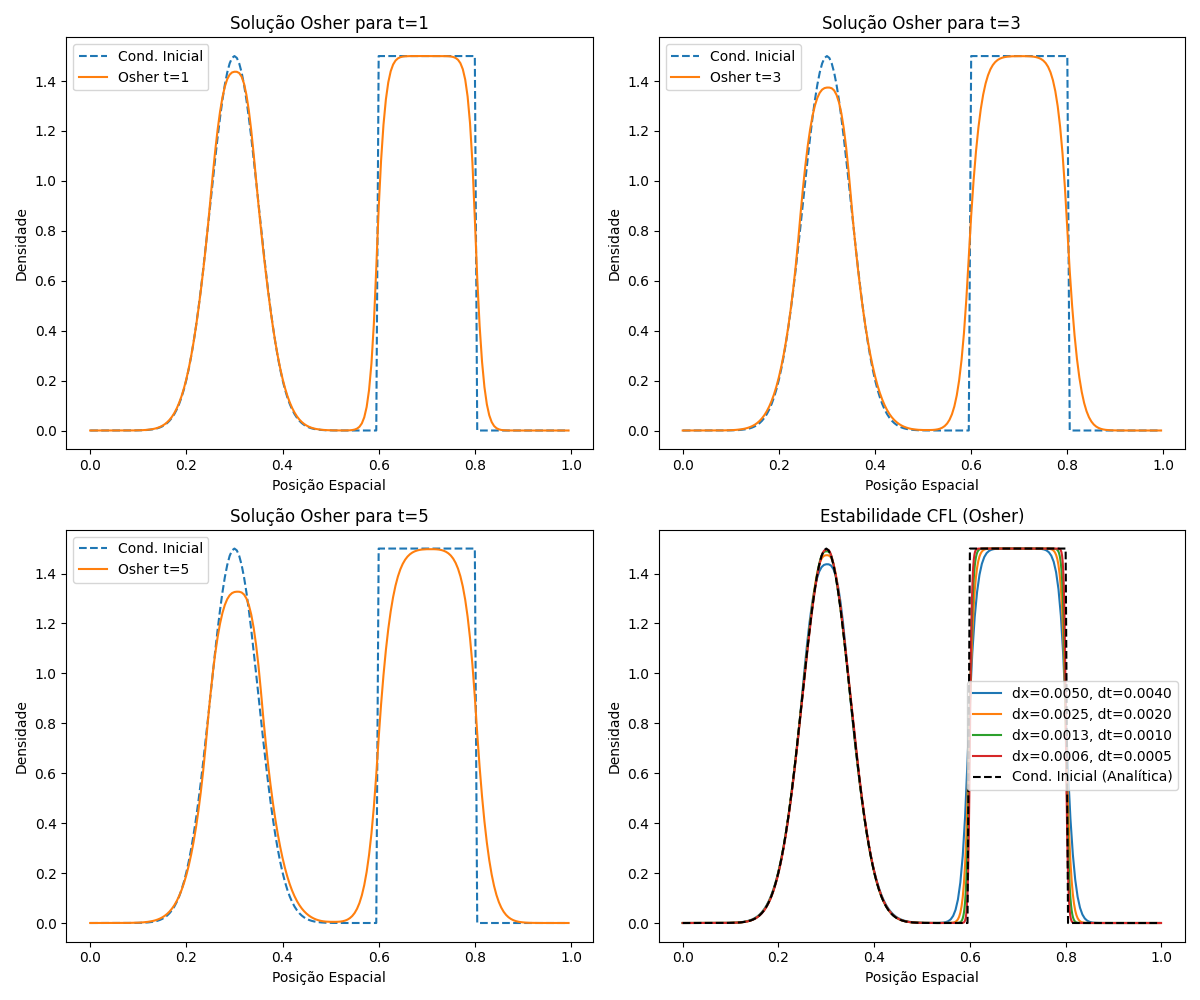
\includegraphics[width=\textwidth]{code/images/Osher.png}
    \caption{Solução Osher para $t=1$, $t=3$ e $t=5$, com a condição inicial representada pela linha tracejada.}
    \label{fig:osher}
\end{figure}

\subsection{Análise dos Resultados do Método Osher}

A Figura \ref{fig:osher} apresenta a evolução da solução obtida pelo método Osher nos tempos \(t=1\), \(t=3\) e \(t=5\), comparando a solução numérica com a condição inicial (\(t=0\)).

- \textbf{Condição inicial (\(t=0\))}: A condição inicial utilizada é uma combinação de uma função gaussiana centrada em \(x=0,3\) e uma concentração uniforme entre \(x=0,6\) e \(x=0,8\).
- \textbf{Incremento de tempo (\(\Delta t\))}: O número de Courant \(C=0,8\) foi aplicado para calcular o passo de tempo, garantindo estabilidade conforme a condição CFL.

Os gráficos mostram que o método Osher preserva de forma eficiente a monotonicidade e a forma geral do perfil de concentração ao longo do tempo, minimizando oscilações. Em \(t=1\), a solução numérica está bem próxima da condição inicial, com pequenas diferenças no topo da gaussiana e nas bordas da concentração uniforme. Para \(t=3\) e \(t=5\), o método continua apresentando um comportamento estável, preservando a forma da gaussiana e do degrau, mas com leves atenuações devido à dissipação numérica.

\begin{table}[H]
    \centering
    \begin{tabular}{rrrrrr}
\toprule
Posicao Espacial & Condicao Inicial & Osher t=1 & Osher t=3 & Osher t=5 & Posicao da Estabilidade \\
\midrule
0.000000 & 0.000000 & 0.000000 & 0.000002 & 0.000006 & 0.000000 \\
0.050000 & 0.000006 & 0.000012 & 0.000034 & 0.000053 & 0.050000 \\
0.100000 & 0.000503 & 0.000718 & 0.001223 & 0.001420 & 0.100000 \\
0.150000 & 0.016663 & 0.018961 & 0.023321 & 0.022593 & 0.150000 \\
0.200000 & 0.203003 & 0.206288 & 0.213317 & 0.192373 & 0.200000 \\
0.250000 & 0.909796 & 0.923582 & 0.967856 & 0.912867 & 0.250000 \\
0.300000 & 1.500000 & 1.437160 & 1.373804 & 1.325958 & 0.300000 \\
0.350000 & 0.909796 & 0.904268 & 0.930223 & 1.030586 & 0.350000 \\
0.400000 & 0.203003 & 0.208248 & 0.218056 & 0.261015 & 0.400000 \\
0.450000 & 0.016663 & 0.019849 & 0.025923 & 0.037466 & 0.450000 \\
0.500000 & 0.000503 & 0.000766 & 0.001917 & 0.004691 & 0.500000 \\
0.550000 & 0.000006 & 0.003678 & 0.028017 & 0.040087 & 0.550000 \\
0.600000 & 1.500000 & 0.890163 & 0.860449 & 0.740881 & 0.600000 \\
0.650000 & 1.500000 & 1.497814 & 1.475949 & 1.438465 & 0.650000 \\
0.700000 & 1.500000 & 1.500000 & 1.499627 & 1.497384 & 0.700000 \\
0.750000 & 1.500000 & 1.498258 & 1.481938 & 1.472013 & 0.750000 \\
0.800000 & 1.500000 & 0.849292 & 0.804179 & 0.905699 & 0.800000 \\
0.850000 & 0.000000 & 0.004615 & 0.036054 & 0.083578 & 0.850000 \\
0.900000 & 0.000000 & 0.000001 & 0.000308 & 0.002432 & 0.900000 \\
0.950000 & 0.000000 & 0.000000 & 0.000003 & 0.000025 & 0.950000 \\
\bottomrule
\end{tabular}

    \caption{Resultados numéricos do método Osher para posições espaciais selecionadas em $t=1$, $t=3$ e $t=5$.}
    \label{tab:osher}
\end{table}

A Tabela \ref{tab:osher} apresenta os valores numéricos da solução do método Osher em posições selecionadas do domínio para diferentes instantes de tempo. Os resultados evidenciam a precisão do método em capturar a evolução do perfil de concentração com o mínimo de oscilações ou dispersão.

\subsection{Implementação em Python}

O código em Python para o método Osher utiliza a função principal \texttt{resolverAdveccaoTVD}, que aplica o limitador e calcula a evolução da densidade ao longo do tempo. A cada passo temporal, o fluxo \(F_{i+1/2}\) é atualizado com base no limitador de Osher, garantindo estabilidade e precisão. O trecho do código é apresentado na Listagem~\ref{lst:codigo_osher}.

\begin{lstlisting}[language=Python, caption={Código para resolver a advecção usando o método Osher}, label={lst:codigo_osher}]
# Método TVD com limitador de Osher
def limitadorOsher(theta):
    return np.maximum(0, np.minimum(1, theta))

def metodoTvdOsher(densidade, nt, intervaloTempo, intervaloEspacial, numeroCourant):
    """
    Método TVD para resolver a advecção utilizando o limitador de Osher.
    """
    for n in range(nt):
        novaDensidade = densidade.copy()
        for i in range(len(densidade)):
            esquerda = (i - 1) % len(densidade)
            direita = (i + 1) % len(densidade)
            # Calcula o gradiente relativo (theta)
            theta = (densidade[i] - densidade[esquerda]) / (densidade[direita] - densidade[i] + 1e-6)
            # Fluxos para direita e esquerda
            fluxoDireita = densidade[i] + 0.5 * numeroCourant * (1 - numeroCourant) * limitadorOsher(theta) * (densidade[direita] - densidade[i])
            fluxoEsquerda = densidade[esquerda] + 0.5 * numeroCourant * (1 - numeroCourant) * limitadorOsher(theta) * (densidade[i] - densidade[esquerda])
            # Atualiza a densidade
            novaDensidade[i] = densidade[i] - numeroCourant * (fluxoDireita - fluxoEsquerda)
        densidade = novaDensidade.copy()
    return densidade
\end{lstlisting}


A implementação do método Osher utiliza o limitador \texttt{limitadorOsher} para controlar os fluxos numéricos em cada passo temporal, garantindo estabilidade e precisão. O número de Courant \(C = 0,8\) é aplicado para satisfazer a condição CFL, essencial para a convergência das soluções numéricas.
 % Done
\subsection{O Método Osher}

O método Osher, baseado no limitador de variação total diminuída (TVD), é projetado para preservar a monotonicidade e minimizar oscilações em regiões com gradientes acentuados. Sua implementação utiliza fluxos numéricos controlados por um limitador, definido como:
\[
    \phi_{\text{lim}}(\theta) = \max(0, \min(1, \theta)),
\]
onde \(\theta\) é uma razão local dos gradientes calculados em cada ponto do domínio.

A solução numérica do método Osher é baseada na atualização iterativa da equação da advecção discretizada em um esquema de volumes finitos:
\[
    Q_i^{n+1} = Q_i^n - C (F_{i+1/2} - F_{i-1/2}),
\]
com o fluxo \(F_{i+1/2}\) controlado pelo limitador \(\phi_{\text{lim}}\).

\begin{figure}[H]
    \centering
    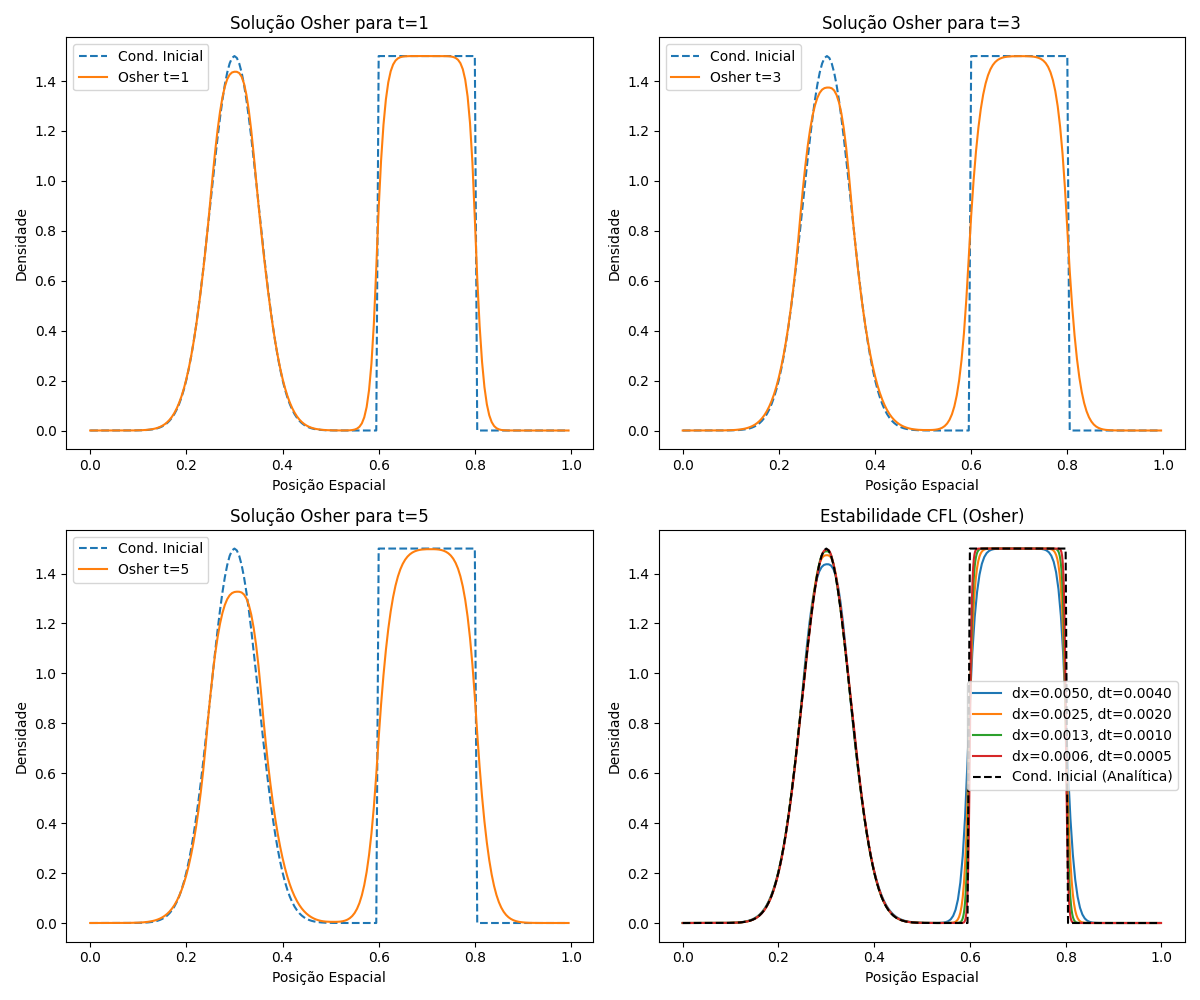
\includegraphics[width=\textwidth]{code/images/Osher.png}
    \caption{Solução Osher para $t=1$, $t=3$ e $t=5$, com a condição inicial representada pela linha tracejada.}
    \label{fig:osher}
\end{figure}

\subsection{Análise dos Resultados do Método Osher}

A Figura \ref{fig:osher} apresenta a evolução da solução obtida pelo método Osher nos tempos \(t=1\), \(t=3\) e \(t=5\), comparando a solução numérica com a condição inicial (\(t=0\)).

- \textbf{Condição inicial (\(t=0\))}: A condição inicial utilizada é uma combinação de uma função gaussiana centrada em \(x=0,3\) e uma concentração uniforme entre \(x=0,6\) e \(x=0,8\).
- \textbf{Incremento de tempo (\(\Delta t\))}: O número de Courant \(C=0,8\) foi aplicado para calcular o passo de tempo, garantindo estabilidade conforme a condição CFL.

Os gráficos mostram que o método Osher preserva de forma eficiente a monotonicidade e a forma geral do perfil de concentração ao longo do tempo, minimizando oscilações. Em \(t=1\), a solução numérica está bem próxima da condição inicial, com pequenas diferenças no topo da gaussiana e nas bordas da concentração uniforme. Para \(t=3\) e \(t=5\), o método continua apresentando um comportamento estável, preservando a forma da gaussiana e do degrau, mas com leves atenuações devido à dissipação numérica.

\begin{table}[H]
    \centering
    \begin{tabular}{rrrrrr}
\toprule
Posicao Espacial & Condicao Inicial & Osher t=1 & Osher t=3 & Osher t=5 & Posicao da Estabilidade \\
\midrule
0.000000 & 0.000000 & 0.000000 & 0.000002 & 0.000006 & 0.000000 \\
0.050000 & 0.000006 & 0.000012 & 0.000034 & 0.000053 & 0.050000 \\
0.100000 & 0.000503 & 0.000718 & 0.001223 & 0.001420 & 0.100000 \\
0.150000 & 0.016663 & 0.018961 & 0.023321 & 0.022593 & 0.150000 \\
0.200000 & 0.203003 & 0.206288 & 0.213317 & 0.192373 & 0.200000 \\
0.250000 & 0.909796 & 0.923582 & 0.967856 & 0.912867 & 0.250000 \\
0.300000 & 1.500000 & 1.437160 & 1.373804 & 1.325958 & 0.300000 \\
0.350000 & 0.909796 & 0.904268 & 0.930223 & 1.030586 & 0.350000 \\
0.400000 & 0.203003 & 0.208248 & 0.218056 & 0.261015 & 0.400000 \\
0.450000 & 0.016663 & 0.019849 & 0.025923 & 0.037466 & 0.450000 \\
0.500000 & 0.000503 & 0.000766 & 0.001917 & 0.004691 & 0.500000 \\
0.550000 & 0.000006 & 0.003678 & 0.028017 & 0.040087 & 0.550000 \\
0.600000 & 1.500000 & 0.890163 & 0.860449 & 0.740881 & 0.600000 \\
0.650000 & 1.500000 & 1.497814 & 1.475949 & 1.438465 & 0.650000 \\
0.700000 & 1.500000 & 1.500000 & 1.499627 & 1.497384 & 0.700000 \\
0.750000 & 1.500000 & 1.498258 & 1.481938 & 1.472013 & 0.750000 \\
0.800000 & 1.500000 & 0.849292 & 0.804179 & 0.905699 & 0.800000 \\
0.850000 & 0.000000 & 0.004615 & 0.036054 & 0.083578 & 0.850000 \\
0.900000 & 0.000000 & 0.000001 & 0.000308 & 0.002432 & 0.900000 \\
0.950000 & 0.000000 & 0.000000 & 0.000003 & 0.000025 & 0.950000 \\
\bottomrule
\end{tabular}

    \caption{Resultados numéricos do método Osher para posições espaciais selecionadas em $t=1$, $t=3$ e $t=5$.}
    \label{tab:osher}
\end{table}

A Tabela \ref{tab:osher} apresenta os valores numéricos da solução do método Osher em posições selecionadas do domínio para diferentes instantes de tempo. Os resultados evidenciam a precisão do método em capturar a evolução do perfil de concentração com o mínimo de oscilações ou dispersão.

\subsection{Implementação em Python}

O código em Python para o método Osher utiliza a função principal \texttt{resolverAdveccaoTVD}, que aplica o limitador e calcula a evolução da densidade ao longo do tempo. A cada passo temporal, o fluxo \(F_{i+1/2}\) é atualizado com base no limitador de Osher, garantindo estabilidade e precisão. O trecho do código é apresentado na Listagem~\ref{lst:codigo_osher}.

\begin{lstlisting}[language=Python, caption={Código para resolver a advecção usando o método Osher}, label={lst:codigo_osher}]
# Método TVD com limitador de Osher
def limitadorOsher(theta):
    return np.maximum(0, np.minimum(1, theta))

def metodoTvdOsher(densidade, nt, intervaloTempo, intervaloEspacial, numeroCourant):
    """
    Método TVD para resolver a advecção utilizando o limitador de Osher.
    """
    for n in range(nt):
        novaDensidade = densidade.copy()
        for i in range(len(densidade)):
            esquerda = (i - 1) % len(densidade)
            direita = (i + 1) % len(densidade)
            # Calcula o gradiente relativo (theta)
            theta = (densidade[i] - densidade[esquerda]) / (densidade[direita] - densidade[i] + 1e-6)
            # Fluxos para direita e esquerda
            fluxoDireita = densidade[i] + 0.5 * numeroCourant * (1 - numeroCourant) * limitadorOsher(theta) * (densidade[direita] - densidade[i])
            fluxoEsquerda = densidade[esquerda] + 0.5 * numeroCourant * (1 - numeroCourant) * limitadorOsher(theta) * (densidade[i] - densidade[esquerda])
            # Atualiza a densidade
            novaDensidade[i] = densidade[i] - numeroCourant * (fluxoDireita - fluxoEsquerda)
        densidade = novaDensidade.copy()
    return densidade
\end{lstlisting}


A implementação do método Osher utiliza o limitador \texttt{limitadorOsher} para controlar os fluxos numéricos em cada passo temporal, garantindo estabilidade e precisão. O número de Courant \(C = 0,8\) é aplicado para satisfazer a condição CFL, essencial para a convergência das soluções numéricas.
 % Done
\subsection{O Método Osher}

O método Osher, baseado no limitador de variação total diminuída (TVD), é projetado para preservar a monotonicidade e minimizar oscilações em regiões com gradientes acentuados. Sua implementação utiliza fluxos numéricos controlados por um limitador, definido como:
\[
    \phi_{\text{lim}}(\theta) = \max(0, \min(1, \theta)),
\]
onde \(\theta\) é uma razão local dos gradientes calculados em cada ponto do domínio.

A solução numérica do método Osher é baseada na atualização iterativa da equação da advecção discretizada em um esquema de volumes finitos:
\[
    Q_i^{n+1} = Q_i^n - C (F_{i+1/2} - F_{i-1/2}),
\]
com o fluxo \(F_{i+1/2}\) controlado pelo limitador \(\phi_{\text{lim}}\).

\begin{figure}[H]
    \centering
    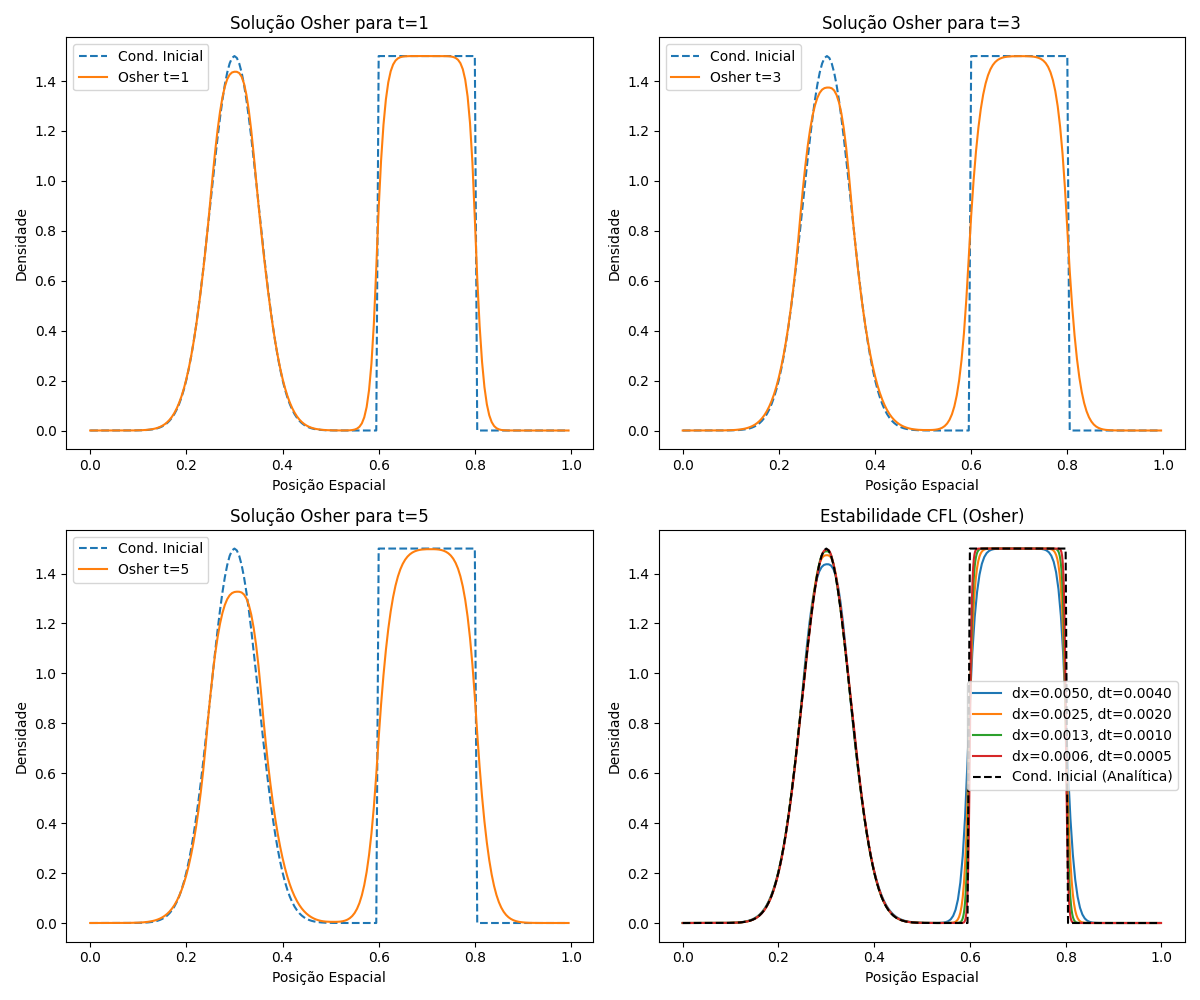
\includegraphics[width=\textwidth]{code/images/Osher.png}
    \caption{Solução Osher para $t=1$, $t=3$ e $t=5$, com a condição inicial representada pela linha tracejada.}
    \label{fig:osher}
\end{figure}

\subsection{Análise dos Resultados do Método Osher}

A Figura \ref{fig:osher} apresenta a evolução da solução obtida pelo método Osher nos tempos \(t=1\), \(t=3\) e \(t=5\), comparando a solução numérica com a condição inicial (\(t=0\)).

- \textbf{Condição inicial (\(t=0\))}: A condição inicial utilizada é uma combinação de uma função gaussiana centrada em \(x=0,3\) e uma concentração uniforme entre \(x=0,6\) e \(x=0,8\).
- \textbf{Incremento de tempo (\(\Delta t\))}: O número de Courant \(C=0,8\) foi aplicado para calcular o passo de tempo, garantindo estabilidade conforme a condição CFL.

Os gráficos mostram que o método Osher preserva de forma eficiente a monotonicidade e a forma geral do perfil de concentração ao longo do tempo, minimizando oscilações. Em \(t=1\), a solução numérica está bem próxima da condição inicial, com pequenas diferenças no topo da gaussiana e nas bordas da concentração uniforme. Para \(t=3\) e \(t=5\), o método continua apresentando um comportamento estável, preservando a forma da gaussiana e do degrau, mas com leves atenuações devido à dissipação numérica.

\begin{table}[H]
    \centering
    \begin{tabular}{rrrrrr}
\toprule
Posicao Espacial & Condicao Inicial & Osher t=1 & Osher t=3 & Osher t=5 & Posicao da Estabilidade \\
\midrule
0.000000 & 0.000000 & 0.000000 & 0.000002 & 0.000006 & 0.000000 \\
0.050000 & 0.000006 & 0.000012 & 0.000034 & 0.000053 & 0.050000 \\
0.100000 & 0.000503 & 0.000718 & 0.001223 & 0.001420 & 0.100000 \\
0.150000 & 0.016663 & 0.018961 & 0.023321 & 0.022593 & 0.150000 \\
0.200000 & 0.203003 & 0.206288 & 0.213317 & 0.192373 & 0.200000 \\
0.250000 & 0.909796 & 0.923582 & 0.967856 & 0.912867 & 0.250000 \\
0.300000 & 1.500000 & 1.437160 & 1.373804 & 1.325958 & 0.300000 \\
0.350000 & 0.909796 & 0.904268 & 0.930223 & 1.030586 & 0.350000 \\
0.400000 & 0.203003 & 0.208248 & 0.218056 & 0.261015 & 0.400000 \\
0.450000 & 0.016663 & 0.019849 & 0.025923 & 0.037466 & 0.450000 \\
0.500000 & 0.000503 & 0.000766 & 0.001917 & 0.004691 & 0.500000 \\
0.550000 & 0.000006 & 0.003678 & 0.028017 & 0.040087 & 0.550000 \\
0.600000 & 1.500000 & 0.890163 & 0.860449 & 0.740881 & 0.600000 \\
0.650000 & 1.500000 & 1.497814 & 1.475949 & 1.438465 & 0.650000 \\
0.700000 & 1.500000 & 1.500000 & 1.499627 & 1.497384 & 0.700000 \\
0.750000 & 1.500000 & 1.498258 & 1.481938 & 1.472013 & 0.750000 \\
0.800000 & 1.500000 & 0.849292 & 0.804179 & 0.905699 & 0.800000 \\
0.850000 & 0.000000 & 0.004615 & 0.036054 & 0.083578 & 0.850000 \\
0.900000 & 0.000000 & 0.000001 & 0.000308 & 0.002432 & 0.900000 \\
0.950000 & 0.000000 & 0.000000 & 0.000003 & 0.000025 & 0.950000 \\
\bottomrule
\end{tabular}

    \caption{Resultados numéricos do método Osher para posições espaciais selecionadas em $t=1$, $t=3$ e $t=5$.}
    \label{tab:osher}
\end{table}

A Tabela \ref{tab:osher} apresenta os valores numéricos da solução do método Osher em posições selecionadas do domínio para diferentes instantes de tempo. Os resultados evidenciam a precisão do método em capturar a evolução do perfil de concentração com o mínimo de oscilações ou dispersão.

\subsection{Implementação em Python}

O código em Python para o método Osher utiliza a função principal \texttt{resolverAdveccaoTVD}, que aplica o limitador e calcula a evolução da densidade ao longo do tempo. A cada passo temporal, o fluxo \(F_{i+1/2}\) é atualizado com base no limitador de Osher, garantindo estabilidade e precisão. O trecho do código é apresentado na Listagem~\ref{lst:codigo_osher}.

\begin{lstlisting}[language=Python, caption={Código para resolver a advecção usando o método Osher}, label={lst:codigo_osher}]
# Método TVD com limitador de Osher
def limitadorOsher(theta):
    return np.maximum(0, np.minimum(1, theta))

def metodoTvdOsher(densidade, nt, intervaloTempo, intervaloEspacial, numeroCourant):
    """
    Método TVD para resolver a advecção utilizando o limitador de Osher.
    """
    for n in range(nt):
        novaDensidade = densidade.copy()
        for i in range(len(densidade)):
            esquerda = (i - 1) % len(densidade)
            direita = (i + 1) % len(densidade)
            # Calcula o gradiente relativo (theta)
            theta = (densidade[i] - densidade[esquerda]) / (densidade[direita] - densidade[i] + 1e-6)
            # Fluxos para direita e esquerda
            fluxoDireita = densidade[i] + 0.5 * numeroCourant * (1 - numeroCourant) * limitadorOsher(theta) * (densidade[direita] - densidade[i])
            fluxoEsquerda = densidade[esquerda] + 0.5 * numeroCourant * (1 - numeroCourant) * limitadorOsher(theta) * (densidade[i] - densidade[esquerda])
            # Atualiza a densidade
            novaDensidade[i] = densidade[i] - numeroCourant * (fluxoDireita - fluxoEsquerda)
        densidade = novaDensidade.copy()
    return densidade
\end{lstlisting}


A implementação do método Osher utiliza o limitador \texttt{limitadorOsher} para controlar os fluxos numéricos em cada passo temporal, garantindo estabilidade e precisão. O número de Courant \(C = 0,8\) é aplicado para satisfazer a condição CFL, essencial para a convergência das soluções numéricas.
 % Done
\section{Desenvolvimento Teórico}

A equação de advecção unidimensional descreve o transporte de uma quantidade conservada, como a concentração de um traçador, ao longo de um eixo espacial. Para resolver essa equação numericamente, é utilizado o método dos Volumes Finitos, que permite a discretização do espaço e do tempo, garantindo uma formulação adequada para a conservação da quantidade transportada \cite{leveque2002finite}. A equação de advecção, em sua forma conservativa, é dada por:

\begin{equation}
    \frac{\partial \Phi}{\partial t} + \frac{\partial}{\partial x} (u \Phi) = 0,
\end{equation}

onde $\Phi$ representa a variável dependente (concentração do traçador) e $u$ é a velocidade de advecção. Com $u$ constante, a equação simplifica-se para:

\begin{equation}
    \frac{\partial \Phi}{\partial t} + u \frac{\partial \Phi}{\partial x} = 0.
\end{equation}

Neste trabalho, a solução numérica é obtida utilizando métodos do tipo \textbf{TVD (Total Variation Diminishing)}. Esses métodos são amplamente reconhecidos por sua capacidade de preservar a monotonicidade da solução e evitar oscilações artificiais, especialmente em regiões com gradientes acentuados ou descontinuidades \cite{harten1983high}. Os métodos implementados são:

\begin{itemize}
    \item \textbf{Limitador de Osher}: Este limitador é projetado para reduzir oscilações artificiais e garantir que a solução permaneça monotônica. Ele é definido como:
          \[
              \phi_{\text{lim}}(\theta) = \max(0, \min(1, \theta)),
          \]
          onde $\theta$ é uma medida da variação local da solução \cite{osher1984rktvd}.

    \item \textbf{Limitador de Sweby}: Este limitador permite maior controle sobre a dissipação, introduzindo um parâmetro ajustável $\beta$. Sua formulação é:
          \[
              \phi_{\text{lim}}(\theta) = \max(0, \min(\beta \theta, \min(1, \theta))),
          \]
          onde valores típicos de $\beta$ estão na faixa $1 \leq \beta \leq 2$ \cite{sweby1984high}.

    \item \textbf{Limitador de Van Albada}: Este limitador equilibra suavidade e precisão, sendo especialmente útil em regiões de gradientes suaves. Sua definição é:
          \[
              \phi_{\text{lim}}(\theta) = \frac{\theta + \theta^2}{1 + \theta^2}.
          \]
          Este limitador é amplamente utilizado devido à sua estabilidade em problemas com gradientes suaves \cite{vanalbada1982family}.
\end{itemize}

Para garantir a estabilidade das simulações, o número de Courant é fixado em $C = 0,8$, respeitando a condição CFL \cite{leveque2002finite}. A condição inicial é definida por uma função composta de uma gaussiana e um valor constante em um intervalo específico, representando um perfil inicial com gradientes suaves e regiões de concentração uniforme. As simulações são realizadas para os instantes de tempo $t = 1$ e $t = 5$, sob condições de contorno periódicas.

Os fluxos nas interfaces dos volumes finitos são calculados considerando os termos anti-difusivos controlados pelos limitadores. A formulação geral do fluxo numérico nos métodos TVD é dada por:
\[
    F_{i+1/2} = u \Phi_i + \frac{u}{2}(1 - C) \phi_{\text{lim}}(\theta_i)(\Phi_{i+1} - \Phi_i),
\]
onde $\theta_i$ é a razão entre os gradientes locais definidos para o intervalo \cite{leveque2002finite}.

Os resultados obtidos serão analisados com gráficos que comparam a solução analítica com as soluções numéricas, permitindo observar a influência de cada limitador na dissipação e dispersão do perfil inicial. Além disso, tabelas apresentarão valores em pontos específicos do domínio para uma análise quantitativa da precisão de cada método.
 % Completa e Validada

% ===============================================================
% Conclusão geral ===============================================
\section{Desenvolvimento Teórico}

A equação de advecção unidimensional descreve o transporte de uma quantidade conservada, como a concentração de um traçador, ao longo de um eixo espacial. Para resolver essa equação numericamente, é utilizado o método dos Volumes Finitos, que permite a discretização do espaço e do tempo, garantindo uma formulação adequada para a conservação da quantidade transportada \cite{leveque2002finite}. A equação de advecção, em sua forma conservativa, é dada por:

\begin{equation}
    \frac{\partial \Phi}{\partial t} + \frac{\partial}{\partial x} (u \Phi) = 0,
\end{equation}

onde $\Phi$ representa a variável dependente (concentração do traçador) e $u$ é a velocidade de advecção. Com $u$ constante, a equação simplifica-se para:

\begin{equation}
    \frac{\partial \Phi}{\partial t} + u \frac{\partial \Phi}{\partial x} = 0.
\end{equation}

Neste trabalho, a solução numérica é obtida utilizando métodos do tipo \textbf{TVD (Total Variation Diminishing)}. Esses métodos são amplamente reconhecidos por sua capacidade de preservar a monotonicidade da solução e evitar oscilações artificiais, especialmente em regiões com gradientes acentuados ou descontinuidades \cite{harten1983high}. Os métodos implementados são:

\begin{itemize}
    \item \textbf{Limitador de Osher}: Este limitador é projetado para reduzir oscilações artificiais e garantir que a solução permaneça monotônica. Ele é definido como:
          \[
              \phi_{\text{lim}}(\theta) = \max(0, \min(1, \theta)),
          \]
          onde $\theta$ é uma medida da variação local da solução \cite{osher1984rktvd}.

    \item \textbf{Limitador de Sweby}: Este limitador permite maior controle sobre a dissipação, introduzindo um parâmetro ajustável $\beta$. Sua formulação é:
          \[
              \phi_{\text{lim}}(\theta) = \max(0, \min(\beta \theta, \min(1, \theta))),
          \]
          onde valores típicos de $\beta$ estão na faixa $1 \leq \beta \leq 2$ \cite{sweby1984high}.

    \item \textbf{Limitador de Van Albada}: Este limitador equilibra suavidade e precisão, sendo especialmente útil em regiões de gradientes suaves. Sua definição é:
          \[
              \phi_{\text{lim}}(\theta) = \frac{\theta + \theta^2}{1 + \theta^2}.
          \]
          Este limitador é amplamente utilizado devido à sua estabilidade em problemas com gradientes suaves \cite{vanalbada1982family}.
\end{itemize}

Para garantir a estabilidade das simulações, o número de Courant é fixado em $C = 0,8$, respeitando a condição CFL \cite{leveque2002finite}. A condição inicial é definida por uma função composta de uma gaussiana e um valor constante em um intervalo específico, representando um perfil inicial com gradientes suaves e regiões de concentração uniforme. As simulações são realizadas para os instantes de tempo $t = 1$ e $t = 5$, sob condições de contorno periódicas.

Os fluxos nas interfaces dos volumes finitos são calculados considerando os termos anti-difusivos controlados pelos limitadores. A formulação geral do fluxo numérico nos métodos TVD é dada por:
\[
    F_{i+1/2} = u \Phi_i + \frac{u}{2}(1 - C) \phi_{\text{lim}}(\theta_i)(\Phi_{i+1} - \Phi_i),
\]
onde $\theta_i$ é a razão entre os gradientes locais definidos para o intervalo \cite{leveque2002finite}.

Os resultados obtidos serão analisados com gráficos que comparam a solução analítica com as soluções numéricas, permitindo observar a influência de cada limitador na dissipação e dispersão do perfil inicial. Além disso, tabelas apresentarão valores em pontos específicos do domínio para uma análise quantitativa da precisão de cada método.


% ===============================================================
% Referencias ===================================================
\section{Desenvolvimento Teórico}

A equação de advecção unidimensional descreve o transporte de uma quantidade conservada, como a concentração de um traçador, ao longo de um eixo espacial. Para resolver essa equação numericamente, é utilizado o método dos Volumes Finitos, que permite a discretização do espaço e do tempo, garantindo uma formulação adequada para a conservação da quantidade transportada \cite{leveque2002finite}. A equação de advecção, em sua forma conservativa, é dada por:

\begin{equation}
    \frac{\partial \Phi}{\partial t} + \frac{\partial}{\partial x} (u \Phi) = 0,
\end{equation}

onde $\Phi$ representa a variável dependente (concentração do traçador) e $u$ é a velocidade de advecção. Com $u$ constante, a equação simplifica-se para:

\begin{equation}
    \frac{\partial \Phi}{\partial t} + u \frac{\partial \Phi}{\partial x} = 0.
\end{equation}

Neste trabalho, a solução numérica é obtida utilizando métodos do tipo \textbf{TVD (Total Variation Diminishing)}. Esses métodos são amplamente reconhecidos por sua capacidade de preservar a monotonicidade da solução e evitar oscilações artificiais, especialmente em regiões com gradientes acentuados ou descontinuidades \cite{harten1983high}. Os métodos implementados são:

\begin{itemize}
    \item \textbf{Limitador de Osher}: Este limitador é projetado para reduzir oscilações artificiais e garantir que a solução permaneça monotônica. Ele é definido como:
          \[
              \phi_{\text{lim}}(\theta) = \max(0, \min(1, \theta)),
          \]
          onde $\theta$ é uma medida da variação local da solução \cite{osher1984rktvd}.

    \item \textbf{Limitador de Sweby}: Este limitador permite maior controle sobre a dissipação, introduzindo um parâmetro ajustável $\beta$. Sua formulação é:
          \[
              \phi_{\text{lim}}(\theta) = \max(0, \min(\beta \theta, \min(1, \theta))),
          \]
          onde valores típicos de $\beta$ estão na faixa $1 \leq \beta \leq 2$ \cite{sweby1984high}.

    \item \textbf{Limitador de Van Albada}: Este limitador equilibra suavidade e precisão, sendo especialmente útil em regiões de gradientes suaves. Sua definição é:
          \[
              \phi_{\text{lim}}(\theta) = \frac{\theta + \theta^2}{1 + \theta^2}.
          \]
          Este limitador é amplamente utilizado devido à sua estabilidade em problemas com gradientes suaves \cite{vanalbada1982family}.
\end{itemize}

Para garantir a estabilidade das simulações, o número de Courant é fixado em $C = 0,8$, respeitando a condição CFL \cite{leveque2002finite}. A condição inicial é definida por uma função composta de uma gaussiana e um valor constante em um intervalo específico, representando um perfil inicial com gradientes suaves e regiões de concentração uniforme. As simulações são realizadas para os instantes de tempo $t = 1$ e $t = 5$, sob condições de contorno periódicas.

Os fluxos nas interfaces dos volumes finitos são calculados considerando os termos anti-difusivos controlados pelos limitadores. A formulação geral do fluxo numérico nos métodos TVD é dada por:
\[
    F_{i+1/2} = u \Phi_i + \frac{u}{2}(1 - C) \phi_{\text{lim}}(\theta_i)(\Phi_{i+1} - \Phi_i),
\]
onde $\theta_i$ é a razão entre os gradientes locais definidos para o intervalo \cite{leveque2002finite}.

Os resultados obtidos serão analisados com gráficos que comparam a solução analítica com as soluções numéricas, permitindo observar a influência de cada limitador na dissipação e dispersão do perfil inicial. Além disso, tabelas apresentarão valores em pontos específicos do domínio para uma análise quantitativa da precisão de cada método.


% ===============================================================
% End Document ==================================================
\end{document}

